The Silicon Photomultiplier (SiPM) is a photosensor, based on semiconductor materials, which has been developed in recent decades and they are replacing conventional PMTs in some experiments or applications. They have been designed to archive outstading photon-counting capabilities better than conventional PMTs with high gain and high photodetection efficiency equal to or larger than conventional PMTs but with some important differences like insensitiveness to magnetic fields, low operating voltage, compactness among other differences.

\textbf{Semiconductor materials} 

Silicon is a semiconductor material and, like any semiconductor material, it has an electronic band structure that consists of two bands: Valence band and conduction band which are separated by a forbidden energy gap (with width of around $1~\eV$ for semiconductors \cite{Leo}) where there cannot be electrons (there are not available energy levels). These energy bands are based on many energy levels that are so close that we can consider a continuum. You can see a diagram of these bands in Figure \ref{fig:EnergyBandsSC}.

\begin{figure}[htbp]
\centering
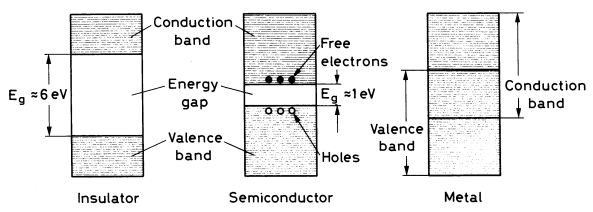
\includegraphics[scale=0.6]{3DesignPrinciples/32Tritium_detector/Energy_bands_isolate_semiconductor_conductor.png}
\caption{Energy band scheme for (a) insulator, (b) semiconductor and (c) conductor.\label{fig:EnergyBandsSC}~\cite{Leo}}
\end{figure}

Electrons in the conduction band, unlike those in the Valence band, can move freely in the material so they contribute to the electric current. 

Silicon has four electrons in their valence band (tetravalent atom) so it form four covalent bounds creating a cristal lattice ($\ce{Si_2}$). Normally a small quantity of impurities ($10^{13}$ atoms/$cm^3$) compared to its density ($10^{22}$ atoms/$cm^3$) are added to modifying this lattice, that's dopping the material. 

If the dopant has 5 valence electrons (pentavalent atom like phosphorus or arsenic) there will be a free electron which will be at an energy level created in the forbbiden band, very close to the conduction band. It is called "n-type" semiconductor and the electrons are the majority charge carriers.

Otherwise, if the dopant has 3 valence atoms (trivalent atom like gallium or boron) it will have a hole\footnote{Electron absence in the crystal lattice} that will be at an energy level created in the forbidden band, very close to the valence band. In this case, the holes are the major charge carriers and this element is called "p-type" semiconductor.

Both configurations (p-type or n-type semiconductor) are shown in the figure \ref{fig:NPType_SC}.

\begin{figure}[htbp]
\centering
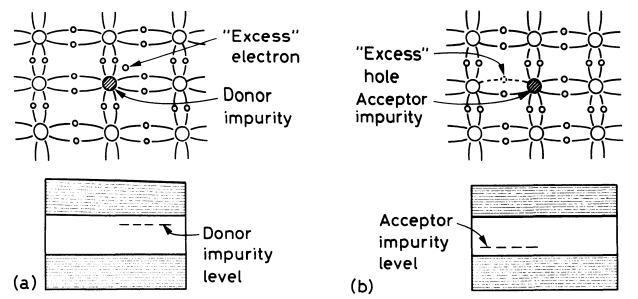
\includegraphics[scale=0.6]{3DesignPrinciples/32Tritium_detector/N_P_type_semiconductors.png}
\caption{Crystal lattice and energy band scheme formed by a silicon with (left) a pentavalent dopant that creates an n-type semiconductor (right) a trivalent dopant that creates a p-type semiconductor. \label{fig:NPType_SC}~\cite{Leo}}
\end{figure}

SiPM is based on a silicon diode formed by a junction of n-type and p-type semiconductors that is made with special techniques to archive a good contact between both surfaces.

This union creates the so-called depletion zone, which is the interface between both materials. In this zone, there are a diffusion of electrons to the p-type semiconductor and holes to the n-type semiconductor due to the difference in the concentration of the majority charge. This re-arrange of the charge creates an electric field in the depletion zone contrary to the movement of these charges, whose potential difference, called contact potential, is $V_0 = 0.7~\volt$ for silicon \cite{Leo}. All this information is shown schematically in the figure \ref{fig:DiodeScheme}

\begin{figure}[htbp]
\centering
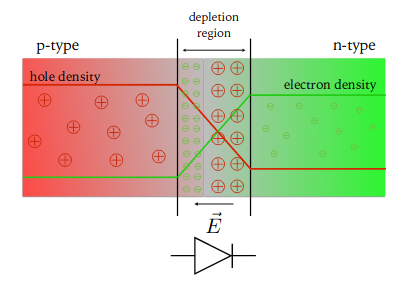
\includegraphics[scale=0.6]{3DesignPrinciples/32Tritium_detector/SchemeSiPMDiodo.png}
\caption{(Above) Schematic of the charge distribution and electric field created in a pn-junction. (Bottom) Commonly used symbol for a diode.\label{fig:DiodeScheme}~\cite{TesisNEXTSiPMs}}
\end{figure}

There are no charge carriers in the depletion zone and, if any one are created, they will be swept out by the electronic field (special interesting property for radiation detectors since charge carriers are created in this zone when ionizing radiation crosses through it).

If we want to use this p-n junction as a particle detector, this setup has some problems that we have to overcome. On the one hand we need to prevent the charge recombination in order to optimize its collection in the depletion zone. On the other hand we need to increase the width of the depletion zone (it is $0.5~\micro\meter$, too small to stop interesting particles) and, as we will see in the section \ref{sec:CharacterizationSiPM}, this small width increases the capacitance value that will increase the electric noise in the output signal.

We can overcome these problems if we apply an external bias voltage across the junction. If this bias voltage is with positive terminal in p-type semiconductor and negative terminal in n-type semiconductor, which is called forward bias voltage, it will create an additional electric field opposite the internal electric field, which will attract electrons in n-type towards p-type and holes in p-type towards n-type. In short, it will reduce the depletion zone, and if the applied voltage is greater than the contact potential, an electric current will be created even if no charge has deposited their energy in the depletion zone.

However, if this bias voltage is applied with positive terminal in n-type semiconductor, negative terminal in p-type semiconductor, which is called reverse bias voltage, the contrary effect will happen and the intensity of the electric field in the depletion zone will be increased. This effect will be limited by the resistence of the semiconductor and if we use a too large bias voltage the pn-juntion will breakdown and it will begin conducting. 

If reverse bias voltage is applied, we can solve all the problems mentioned above. In this case, the charge collection will be improved and the width of the depletion zone will be increased. If ionizing radiation crosses the depletion zone, which is wide enough to detect interesting particles, it will deposit their energy and, due to that, charge charriers will be created\footnote{The energy required to create an electron-hole pair in silicon is $3.62~\eV$ in STP\cite{Leo}} which will be swept due to the electric field and an optimized current signal will be created. 

Depending on the intensity of the polarization voltage we can work in different modes and we will have different output signals. If the bias voltage is less than the threshold, the charge carriers will recombine and no output signal will be produced. If the bias voltage is larger than threshold an avalanche is created due to each original electron and it is independent of other possible avalenches. Due to this avalanche, it has a gain whose valuer is around $200$. This mode is called proportional mode since the collected charged is proportional to the energy deposited. Finally, If the bias voltage is even larger, each avalanche can trigger a second avalanche and, due to that, their internal gain is higher than the proportional mode\footnote{The gain of commercial SiPMs, for example Hammamatsu, is of the order of $10^6$, similar to the PMTs}, that's, it's output signal will be larger. This mode is called Geiger mode since the output signal only show when a detection has happened but it is not proporcional to the energy deposited. 

The voltage at which the SiPM changes from proportional to geiger mode is called the breakdown voltage, $ V_ {BR} $. If it works at a lower voltage it is in proportional mode but if it works at a higher voltage, it works in geiger mode. The measurement of the breakdown voltage is one of the most important things to characterize the SiPM and I show how we have done it in the section \ref{sec:CharacterizationSiPM}.

\textbf{Silicon photomultiplier}

The SiPM is based on a matrix of APDs which are photodiodes operating in geiger mode. A scheme of an APD used in a SiPM is shown in the figure \ref{fig:SchemeAPD}. It has p+ and a n+ layers\footnote{p+ and n+ layers are the same as p and n layers, explained before, but with higher concentrations of acceptor impurities or donor impurities respectively CHECK THAT!!} that are used because they improve the properties of SiPMs but the way these APDs work is the same as that described before. 

\begin{figure}[htbp]
\centering
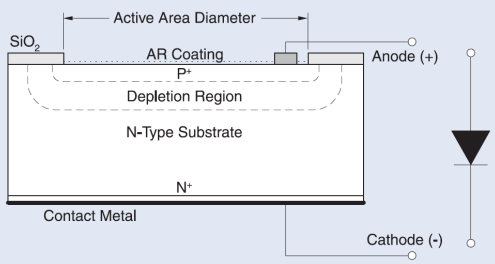
\includegraphics[scale=0.6]{3DesignPrinciples/32Tritium_detector/APD_scheme.png}
\caption{Scheme of a APD and electrical symbol used.\label{fig:SchemeAPD}~\cite{OSI}}
\end{figure}
 
These APDs, called pixels when they are part of a SiPM, are connected in parallel and we read the sum of all of them at each moment. The output signal of each pixel is approximately the same regardless of the energy deposited, with some difference due to the uncertainty in the SiPM manufacturing process and the statistical nature of the detection process. Due to that, we cannot know the energy deposited in each APD but, as we read all SiPM pixels at the same time, the charge of the output signal when we detect n photons simultaneously will be n times the charge we have when we detect only one photon, as can be seen in figure \ref{fig:PulsesOfSiPM}. Due to this property, after a correct calibration of our SiPMs which will be shown in the section \ref{sec:CharacterizationSiPM}, we can know how many photons we have detected, which have a linear relationship with the output signal. 

Furthermore, as we saw in section \ref{subsec:PlasticScintillators}, since we work with scintillators, in our case, the number of photons is proportional to the deposited energy, so we can recover the characteristic linearity of its output signal and to know the energy deposited in our scintillator, and, therefore, the energy of the initial radioactive event.

\begin{figure}[htbp]
\centering
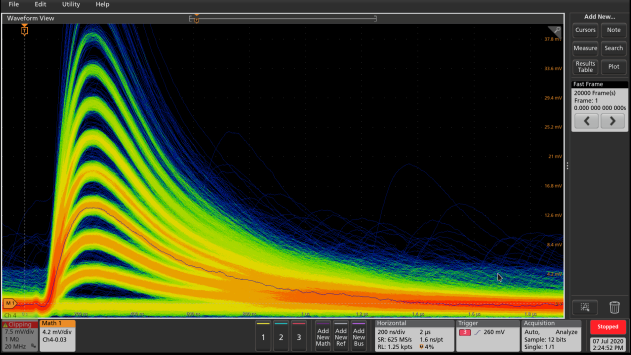
\includegraphics[scale=0.6]{3DesignPrinciples/32Tritium_detector/Several_SiPM_pulses.png}
\caption{Using persistence on the oscilloscope to show several pulses with different heights. Each height associated with a different number of  SiPM pixels lit at the same time.\label{fig:PulsesOfSiPM}}
\end{figure}

On top of that, these pixels need to be so small\footnote{Pixel sizes for commercial SiPMs are $50$ or $75\mu\meter$ \cite{DataSheetHammamatsu_1_SiPM_50}, \cite{DataSheetHammamatsu_1_SiPM_75}} that, if the photon density to be detected is low enough, we only detect one photon in each pixel. If it doesn't happen, we will detect two or more photons with the same pixel but the output signal will be the same as one detected photon, so we will have a loss of linearity of our output signal. This effect is known as saturation and it is important to know the photon density at which it happens for our SiPMs. The experimental measurements of this effect, which have been done for our SiPMs, is shown in the section \ref{sec:CharacterizationSiPM}. SI LA MIDO YO PERFECTO, SI NO DECIR QUE PARA NEUSTRO CASO NO ES IMPORTANTE PORQEU ESTAMOS MIDIENDO MUY POCOS FOTONES POR EVENTO.

Each of these pixels has a quenching resistance\footnote{The tipical valuer of this quenching resistance for commercial SiPMs is around $500~\kilo\Omega$} in series that is used to stop the current produced when this pixel has detected a particle. It is used for limit the current drawn by the diode during breakdown and reduce the reverse voltage seen by the diode to one below the breakdown voltage. After that, the voltage seen by the diode is reset to the bias voltage and this pixel is ready to detect a new particle again. In figure \ref{fig:ChenchingResistance} (left) a diagram of these chenching resistances and APDs in a SiPM and (right) how it works is shown respectively.

\begin{figure}[htbp]
\centering
{
%\subfloat[PDE]
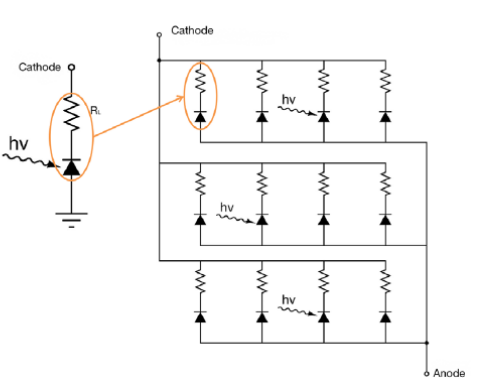
\includegraphics[scale=0.35]{3DesignPrinciples/32Tritium_detector/Quenching_resistence_of_a_SiPM_scheme.png}
%\caption{Simple electronic model of a SiPM.\label{fig:ElectricModelSiPM}~\cite{DataSheetSensL}}
}
{
%\subfloat[Espectro de emisión]
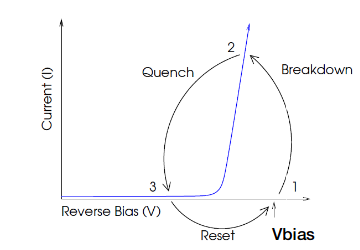
\includegraphics[scale=0.5]{3DesignPrinciples/32Tritium_detector/How_a_quenching_resistence_in_a_SiPM_works.png}
%\caption{Output current of a SiPM as a function of the reverse voltage. It show that the quenching mechanism is essential for working with SiPMs\label{fig:HowSiPMworks}~\cite{DataSheetSensL}}
}
\caption{(Left) Electronic scheme of a SiPM and (right) output current of a SiPM as a function of the reverse voltage. It show that the quenching mechanism is essential for working with SiPMs\label{fig:ChenchingResistance}~\cite{DataSheetSensL}}
\end{figure}

In this simple electrical scheme we can see that all pixels have a common cathode and anode which means that, as we said before, they are at the same bias voltage and the output is the sum of all of them.

We have a lot of names to refer to these photosensors such as SiPMs, MPPCs, G-APDs, SSPMs, MRS-ADPs or AMPDs. The candidate for TRITIUM project is S13360-6075 from Hamamatsu photonics \cite{DataSheetHammamatsu_1_SiPM_75} because its characteristics are the ones that best fit our objectives since this model has super low afterpulses, crosstalk and dark counts than other SiPM models from Hammamatsu. Its characteristics and properties are shown in the table \ref{tab:PropertiesOfSiPM75}. 

\begin{table}[htbp]
%%\centering.
\begin{center}
\begin{tabular}{|c|c|}
\hline
Parameter & Numerical value \\
\hline \hline \hline
Serie & $S13360$ \\ \hline
Model & $6075$ \\ \hline
Pixel Pitch ($\mu\meter$) & $75$ \\ \hline
Effective photosensitive area ($\mm^2$) & $6.0 \times 6.0$ \\ \hline
Number of pixels & $6400$ \\ \hline
Fill factor & $82\%$ \\ \hline
Refractive index of windows material & $1.55$ \\ \hline
Operating temperature range ($\degree C$)& $[-20,60]$ \\ \hline
Spectral response range, $\lambda$ ($\nano\meter$) & $[320, 900]$ \\ \hline
Peak sensitivity wavelength, $\lambda_p$ ($\nano\meter$) & $450$ \\ \hline
PhotoDetection Efficiency, PDE, $\lambda=\lambda_p$ ($\%$) & $50$ \\ \hline
Dark counts, Typical/Maximum (kcps) & $2000/6000$ \\ \hline
Terminal capacitance, $C_t$ ($\pico\farad$) & $1280$ \\ \hline
Gain, M, & $4 \cdot{} 10^6$ \\ \hline
Breakdown Voltage, $V_{BR}$ ($\volt$) & $53$ \\ \hline
Cross talk probability($\%$) & $7$ \\ \hline
Temperature coefficient $\Delta TV_{op}$ (m$\volt/\degree C$) & $54$ \\ \hline
\end{tabular}
\caption{Characteristics of SiPM S13360-6075 from Hammamatsu Photonics \cite{DataSheetHammamatsu_1_SiPM_75}.}
\label{tab:PropertiesOfSiPM75}
\end{center}
\end{table}

These characteristics and properties will be explained and their experimental measurements will be shown in section \ref{sec:CharacterizationSiPM}. These numerical values, which appear in the table \ref{tab:PropertiesOfSiPM75}, are provided by Hammamatsu photonics but it is only an approximation for this model. These parameters must be determined experimentally for each SiPM used because it can be very different even if it is the same model.

It must be taken into account that we will do this characterization at the level of a single SiPM because, at the beginning, it is easier to understand the results but we will work with a matrix of them and we will have to do this characterization for each matrix used. 

The matrices under consideration are the model "S13361-6050" from Hammamatsu, which consists of a $4\times 4$ SiPM matrix where the active area of each SiPM is $6\times 6~\mm$ \cite{DataSheetHammamatsu_array_SiPM_6050} or the model "S13361-3050" from Hammamatsu, which consists of a $8\times 8$ SiPM where the active area of each is $3\times 3~\mm$ \cite{DataSheetHammamatsu_array_SiPM_3050}. They are a commercial matrices from Hammamatsu and, as you can see, the total active area that we will cover with these arrangements is the same in both cases, $24\times 24~\mm$ and it is approximatelly the same that the active area covered with the PMTs used, which has been shown in the previous section.

These matrices have a common bias voltage and common ground for all SiPMs that are contained and we will have an output signal for each SiPM. 

We hope to obtain better results with the 4x4 matrix for theoretical reasons which we will see in the section \ref{sec:CharacterizationSiPM} like larger PDE, mainly due to a larger active area but it is something that we will have to verify with experimental measurements.




Nuestro SiPM esta dopado? con que?